% fhsm_2009_p58_2.tex
\documentclass[tikz,border=6pt]{standalone}
\usetikzlibrary{calc,angles,quotes,arrows.meta}

\begin{document}
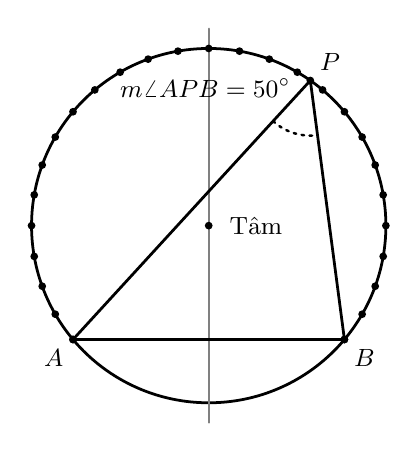
\begin{tikzpicture}[font=\small,line cap=round,line join=round,>=Stealth]

% ----- circle + points -----
\def\R{2.25}
\coordinate (O) at (0,0);

% points on the circle (match layout: A left-lower, B right-lower, P upper-right)
\coordinate (A) at ($(O)+(220:\R)$);
\coordinate (B) at ($(O)+(320:\R)$);
\coordinate (P) at ($(O)+(55:\R)$);

% ----- circle outline -----
\draw[line width=1.0pt] (O) circle (\R);

% ----- axes (vertical diameter emphasized; small cross at top like in scan) -----
\draw[line width=.8pt, color=gray] (0,\R+0.25) -- (0,-\R-0.25);
% \draw[line width=1.0pt] (-0.25,\R) -- (0.25,\R);

% ----- triangle APB -----
\draw[line width=1.0pt] (A) -- (B) -- (P) -- cycle;

% ----- points + labels -----
\fill (A) circle (1.4pt) node[below left] {$A$};
\fill (B) circle (1.4pt) node[below right] {$B$};
\fill (P) circle (1.4pt) node[above right] {$P$};

% center point + label
\fill (O) circle (1.4pt);
\node[right=4pt] at (O) {Tâm};

% ----- dotted MAJOR arc from A to B (only the top arc; no extra arc below) -----
% With O above AB, A has polar angle 220°, B has 320° (relative to O).
% The MAJOR arc goes 220 -> 360 -> 320.
\foreach \ang in {220,210,...,90,80,70,...,0,350,340,...,320}{
  \fill ($(O)+(\ang:\R)$) circle (1.4pt);
}

% ----- angle marker at P (50°) -----
\pic[
  draw,
  dotted,
  line width=0.9pt,
  angle radius=7mm,
  angle eccentricity=1.05
] {angle=A--P--B};

\node[anchor=west] at (-1.25,1.75) {$m\angle APB=50^\circ$};


\end{tikzpicture}
\end{document}
